\section{Software-based Error Coding}
\label{sec:ErrorCoding}

Our novel \emph{AHEAD} approach is based on error coding instead of general-purpose DMR. The most important property of error codes is the detection capability, i.e. the guaranteed minimum bit flip weight, whereby the basic idea is as follows: The data word space $\mathbb{D}$ contains the original data. From a given \emph{data word} an encoding (hardening) maps to a \emph{code word}, which can be decoded back (softening) to the original data word in the best case without bit flips. The code domain is typically much larger than the original data domain, where only the original data words can be mapped between both domains. The code words belonging to this subset are called \emph{valid} -- valid hardened data words. All other code words are \emph{invalid} or \emph{corrupted}. A bit flip may change a valid code word either to an invalid one which can be detected, or to another valid one which is undetectable and known as silent data corruption (SDC). 

Error codes have been widely studied in theory and applied in practice~\cite{moon2005error}. Thus, there is a large corpus of error codes available~\cite{moon2005error}. We examined a variety of these codes with regard to our three requirements \textbf{R1} to \textbf{R3}. Based on this analysis, we decided to use an arithmetic code called \emph{AN coding}. Before we justify our decision in Section~\ref{sec:ANCodingJustification}, we introduce AN coding in detail in Section~\ref{sec:ANCodingDescription}. Figure~\ref{fig:hamming-an-illustration} highlights and compares AN coding (right side) with the well-known Hamming code~\cite{hamming1950error} (left) using an $8$-bit example value.  
 

\subsection{AN Coding Description}
\label{sec:ANCodingDescription}

AN coding is a representative of arithmetic codes\footnote{Please note that some unrelated codes for lossless lightweight data compression are also called arithmetic codes~\cite{DBLP:journals/cacm/WittenNC87}. These are \emph{not} equivalent to the codes used here.}~\cite{DBLP:journals/tc/Avizienis71,DBLP:conf/hase/HoffmannUDSLS14}, allowing only error detection. Hardened code words \(c\in\mathbb{C}_{\mathbb{D}_\Theta}^A\) are computed by multiplying a constant \(A\in\mathbb{A}\) onto each original data word \(d\in\mathbb{D}_\Theta\) as illustrated on the right side in Figure~\ref{fig:hamming-an-illustration}:
\vspace{-0.1cm}
 \begin{align}
c &= d \cdot A \label{eq:ANencode}
\vspace{-0.1cm}
\end{align}
\(\mathbb{A}\), \(\mathbb{D}_\Theta\), and \(\mathbb{C}_{\mathbb{D}_\Theta}^A\) respectively are the sets of all possible parameters \(A\), data words \(d\) of type \(\Theta\), and code words \(c\). The multiplication modifies the data word itself and all data is viewed as integers. As a result of the multiplication, the domain of code words \(\mathbb{C}_{\mathbb{D}_\Theta}^A\) expands such that only multiples of \(A\) become valid code words, and all other integers are considered non-code words. The impact of \(A\) on the detection capability is described later. A division is required for softening:
\vspace{-0.1cm}
\begin{align}
d &= c / A \label{eq:ANdecode}
\vspace{-0.1cm}
\end{align}
Errors are detected by testing the remainder of the division by \(A\), which must be zero, otherwise the code word was corrupted (\(c_\varepsilon\)), e.g., by a bit flip denoted as \(b\):
\vspace{-0.1cm}
\begin{align}
c &\equiv 0 \quad (\text{mod }A) \label{eq:ANcheck} \\
(c_\varepsilon = c \oplus\footnotemark b) &\not\equiv 0 \quad (\text{mod }A) \label{eq:ANcheckerror}
\end{align}
\footnotetext{\(\oplus\) can be a binary XOR, OR, or AND-operation, depending on the actual error model.}
A unique feature of arithmetic codes, and thus AN coding, is the ability to operate directly on hardened data by encoding the other operands, too. In particular, due to the monotony of the multiplication, the following operations on two hardened operands yield the same results as operations on unencoded data:
\begin{align}
c_1 \pm c_2 & = (d_1 \cdot A) \pm (d_2 \cdot A) = (d_1 \pm d_2) \cdot A \label{eq:ANPlusMinus} \\
c_1 \circ c_2 & \equiv (d_1 \cdot A) \circ (d_2 \cdot A) \myequiv{\nicefrac[\texttt]{1}{A}} d_1 \circ d_2 \text{~,~} \circ\in\{<, \leq, =, \dots\} \label{eq:ANCompare}
\end{align}

Care must be taken for operations like multiplication
\begin{subequations}
\begin{align}
	\text{OK} \quad c_1 \cdot d_2 &= d_1 \cdot d_2 \cdot A,
	\label{eq:ANMulUnenc}
	\\
	\text{BAD} \quad c_1 \cdot c_2 &= (d_1 \cdot A) \cdot (d_2 \cdot A) = d_1 \cdot d_2 \cdot A^2,
	\label{eq:ANMulBad}
	\\
	\text{OK} \quad c_1 \cdot c_2 &\Rightarrow c_1 \cdot \nicefrac{c_2}{A} = d_1 \cdot d_2 \cdot A,
	\label{eq:ANMulOK}
\end{align}
\end{subequations}
and division
\begin{subequations}
\begin{align}
	\text{OK} \quad \frac{c_1}{d_2} &= \frac{d_1 \cdot A}{d_2} = \frac{d_1}{d_2} \cdot A,
	\label{eq:ANDivUnenc}
	\\
	\text{BAD} \quad \frac{c_1}{c_2} &= \frac{d_1 \cdot A}{d_2 \cdot A} = \frac{d_1}{d_2},
	\label{eq:ANDivBad}
	\\
	\text{OK} \quad \frac{c_1}{c_2} &\Rightarrow \frac{c_1}{c_2} \cdot A = \frac{d_1 \cdot A}{d_2 \cdot A} \cdot A = \frac{d_1}{d_2} \cdot A.
	\label{eq:ANDivOK}
\end{align}
\end{subequations}
While \Cref{eq:ANMulUnenc,eq:ANDivUnenc} are valid operations using an encoded and an unencoded operand, \Cref{eq:ANMulBad}'s result would be invalid due to the resulting \(A^2\) and \Cref{eq:ANDivBad} produces an unencoded result. By that, for multiplication with two hardened operands, one operand must be divided by \(A\) (\Cref{eq:ANMulOK}). For division, the result must be multiplied by \(A\) (\Cref{eq:ANDivOK}), where the correct order of the additional multiplication is crucial. The division of the two code words must take precedence to prevent an overflow.

\begin{figure}
	\centering
	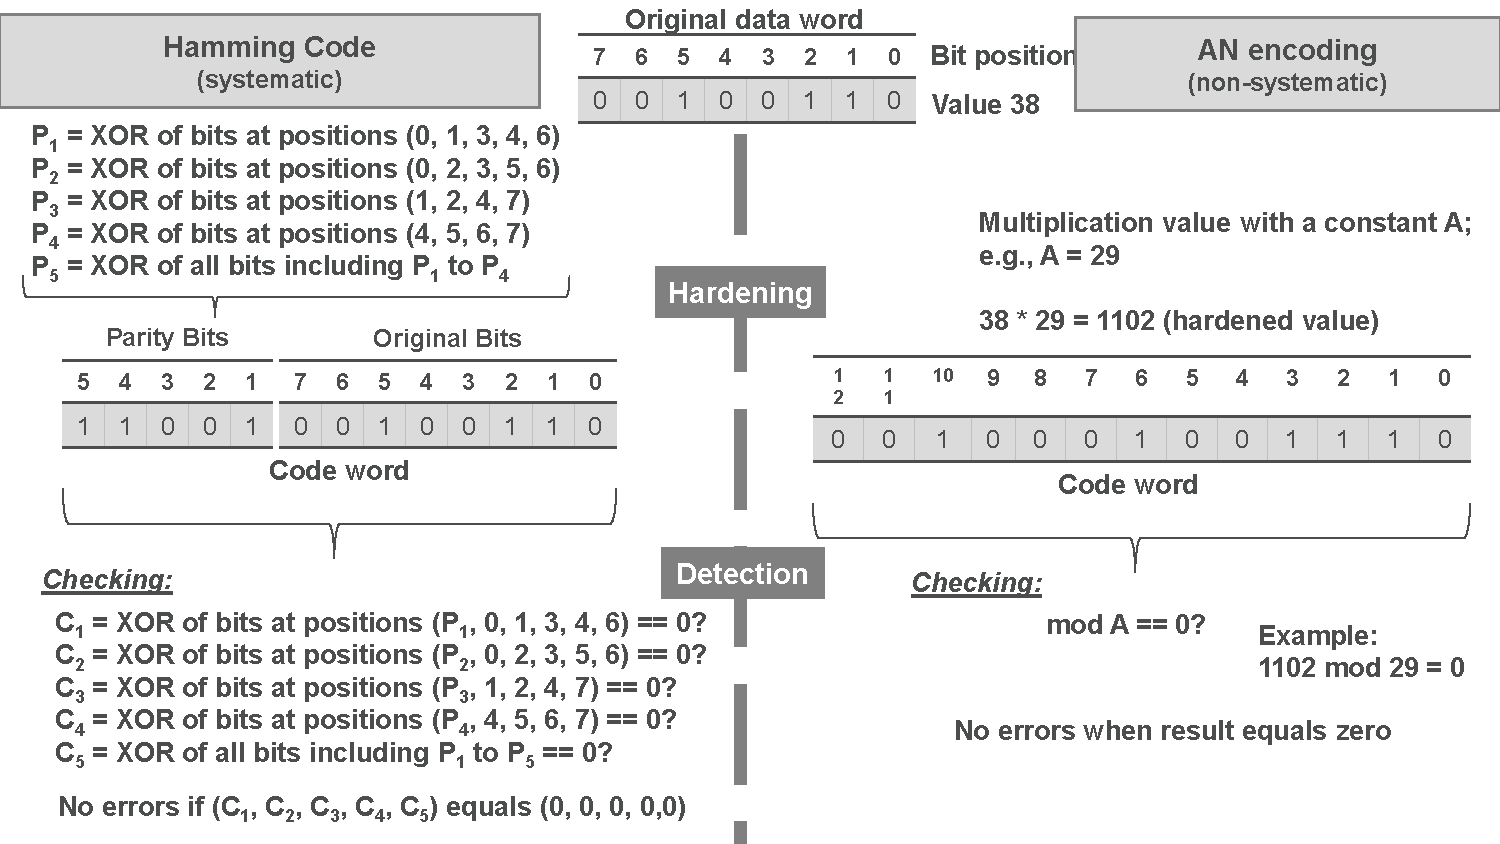
\includegraphics[width=\linewidth]{figures/hamming-an-illustration.pdf}	
	\vspace{-0.5cm}
	\caption{Illustration of Hamming and AN coding.}% using an $8$-bit value. In both cases, the hardened data words require $13$ bits and up to $2$ arbitrary bit flips are completely detectable.} 
	\label{fig:hamming-an-illustration}
	\vspace{-0.4cm}
\end{figure}


\subsection{AN Coding Justification}
\label{sec:ANCodingJustification}

As shown in Figure~\ref{fig:hamming-an-illustration}, AN coding hardens the bit representation of the original value with additional bits for error detection. This applies not only to AN coding, but also to any other error code~\cite{moon2005error}. For example, the left side of Figure~\ref{fig:hamming-an-illustration} shows the hardening using the well-known Extended Hamming code~\cite{hamming1950error}. As illustrated, the Extended Hamming Code also introduces five additional parity bits as AN coding in this setting, whereas four are computed using a bit mask (not shown here for brevity, but indicated in Figure~\ref{fig:hamming-an-illustration}) over the $8$-bit value. The fifth parity bit $P_5$ is computed over all bits. 

A difference between both codes is that AN coding is a representative of \emph{non-systematic error codes}, whereas Hamming is a \emph{systematic error code}. Systematic codes allow a separation of the original bits and additional bits. This means that the original data word is embedded as-is in the hardened representation (cf. Figure~\ref{fig:hamming-an-illustration}). In contrast, in non-systematic codes, the hardened representation does not contain the original data, so that it is not separable from the additional bits. While this makes accessing the original data faster, AN codes have a big advantage: the hardened codewords can be processed directly and each arithmetic operation also computes the additional bits, which is not the case for codes like Hamming. There, the additional bits have to be recomputed in addition to each arithmetic, introducing even more computational overhead. By that, for the database domain, codes like AN codes are preferable. Furthermore, the complete and direct processing of the hardened codewords as possible for AN codes allows the recognition of (i) errors that modify data stored in memory, (ii) errors induced during transferring on interconnects, and (iii) errors induced during computations (satisfying requirement \textbf{R1}). 

In our example (Figure~\ref{fig:hamming-an-illustration}), the specific AN code with $A=29$ and the Extended Hamming code introduce five additional bits. Both codes detect all $1$- and $2$-bit flips per code word, but in contrast to AN codes, Extended Hamming can also \emph{correct} $1$-bit errors. However, the correction property has a negative impact on the error detection capability for bit flips weights $\geq 2$ (cf. Figure~\ref{fig:8bitSDCProbability}). The chances of \emph{detecting} higher bit flip weights are much better for AN coding than for Hamming, because the SDC probability\footnote{The computation of these SDC probabilities is a topic of its own and described in Appendix~\ref{appendix:SDCProbability}} is much lower. As depicted in Figure~\ref{fig:8bitSDCProbability}, Hamming shows a zig\=zag\=curve for higher bit flip weights due to the correction capabilities and this pattern holds for all Hamming codes. Many invalid code words resulting from odd\=numbered bit flip weights ($>2$) are mistakenly corrected to a different data word, which is not detectable. Server-grade ECC main memory uses Hamming codes and thus exhibits such behavior. This is another reason for employing AN codes for \emph{detection} and why we concentrate on detection in this paper.

\begin{figure}
	\centering
	{
		\scriptsize
		\graphicspath{{gnuplot/}}
		% GNUPLOT: LaTeX picture with Postscript
\begingroup
  \makeatletter
  \providecommand\color[2][]{%
    \GenericError{(gnuplot) \space\space\space\@spaces}{%
      Package color not loaded in conjunction with
      terminal option `colourtext'%
    }{See the gnuplot documentation for explanation.%
    }{Either use 'blacktext' in gnuplot or load the package
      color.sty in LaTeX.}%
    \renewcommand\color[2][]{}%
  }%
  \providecommand\includegraphics[2][]{%
    \GenericError{(gnuplot) \space\space\space\@spaces}{%
      Package graphicx or graphics not loaded%
    }{See the gnuplot documentation for explanation.%
    }{The gnuplot epslatex terminal needs graphicx.sty or graphics.sty.}%
    \renewcommand\includegraphics[2][]{}%
  }%
  \providecommand\rotatebox[2]{#2}%
  \@ifundefined{ifGPcolor}{%
    \newif\ifGPcolor
    \GPcolortrue
  }{}%
  \@ifundefined{ifGPblacktext}{%
    \newif\ifGPblacktext
    \GPblacktexttrue
  }{}%
  % define a \g@addto@macro without @ in the name:
  \let\gplgaddtomacro\g@addto@macro
  % define empty templates for all commands taking text:
  \gdef\gplbacktext{}%
  \gdef\gplfronttext{}%
  \makeatother
  \ifGPblacktext
    % no textcolor at all
    \def\colorrgb#1{}%
    \def\colorgray#1{}%
  \else
    % gray or color?
    \ifGPcolor
      \def\colorrgb#1{\color[rgb]{#1}}%
      \def\colorgray#1{\color[gray]{#1}}%
      \expandafter\def\csname LTw\endcsname{\color{white}}%
      \expandafter\def\csname LTb\endcsname{\color{black}}%
      \expandafter\def\csname LTa\endcsname{\color{black}}%
      \expandafter\def\csname LT0\endcsname{\color[rgb]{1,0,0}}%
      \expandafter\def\csname LT1\endcsname{\color[rgb]{0,1,0}}%
      \expandafter\def\csname LT2\endcsname{\color[rgb]{0,0,1}}%
      \expandafter\def\csname LT3\endcsname{\color[rgb]{1,0,1}}%
      \expandafter\def\csname LT4\endcsname{\color[rgb]{0,1,1}}%
      \expandafter\def\csname LT5\endcsname{\color[rgb]{1,1,0}}%
      \expandafter\def\csname LT6\endcsname{\color[rgb]{0,0,0}}%
      \expandafter\def\csname LT7\endcsname{\color[rgb]{1,0.3,0}}%
      \expandafter\def\csname LT8\endcsname{\color[rgb]{0.5,0.5,0.5}}%
    \else
      % gray
      \def\colorrgb#1{\color{black}}%
      \def\colorgray#1{\color[gray]{#1}}%
      \expandafter\def\csname LTw\endcsname{\color{white}}%
      \expandafter\def\csname LTb\endcsname{\color{black}}%
      \expandafter\def\csname LTa\endcsname{\color{black}}%
      \expandafter\def\csname LT0\endcsname{\color{black}}%
      \expandafter\def\csname LT1\endcsname{\color{black}}%
      \expandafter\def\csname LT2\endcsname{\color{black}}%
      \expandafter\def\csname LT3\endcsname{\color{black}}%
      \expandafter\def\csname LT4\endcsname{\color{black}}%
      \expandafter\def\csname LT5\endcsname{\color{black}}%
      \expandafter\def\csname LT6\endcsname{\color{black}}%
      \expandafter\def\csname LT7\endcsname{\color{black}}%
      \expandafter\def\csname LT8\endcsname{\color{black}}%
    \fi
  \fi
    \setlength{\unitlength}{0.0500bp}%
    \ifx\gptboxheight\undefined%
      \newlength{\gptboxheight}%
      \newlength{\gptboxwidth}%
      \newsavebox{\gptboxtext}%
    \fi%
    \setlength{\fboxrule}{0.5pt}%
    \setlength{\fboxsep}{1pt}%
\begin{picture}(4600.00,1720.00)%
    \gplgaddtomacro\gplbacktext{%
      \csname LTb\endcsname%
      \put(604,563){\makebox(0,0)[r]{\strut{}\tiny{\num{0.01}}}}%
      \csname LTb\endcsname%
      \put(604,955){\makebox(0,0)[r]{\strut{}\tiny{\num{0.1}}}}%
      \csname LTb\endcsname%
      \put(604,1347){\makebox(0,0)[r]{\strut{}\tiny{\num{1}}}}%
      \csname LTb\endcsname%
      \put(909,272){\makebox(0,0){\strut{}$1$}}%
      \csname LTb\endcsname%
      \put(1100,272){\makebox(0,0){\strut{}$2$}}%
      \csname LTb\endcsname%
      \put(1292,272){\makebox(0,0){\strut{}$3$}}%
      \csname LTb\endcsname%
      \put(1483,272){\makebox(0,0){\strut{}$4$}}%
      \csname LTb\endcsname%
      \put(1675,272){\makebox(0,0){\strut{}$5$}}%
      \csname LTb\endcsname%
      \put(1866,272){\makebox(0,0){\strut{}$6$}}%
      \csname LTb\endcsname%
      \put(2058,272){\makebox(0,0){\strut{}$7$}}%
      \csname LTb\endcsname%
      \put(2249,272){\makebox(0,0){\strut{}$8$}}%
      \csname LTb\endcsname%
      \put(2441,272){\makebox(0,0){\strut{}$9$}}%
      \csname LTb\endcsname%
      \put(2632,272){\makebox(0,0){\strut{}$10$}}%
      \csname LTb\endcsname%
      \put(2824,272){\makebox(0,0){\strut{}$11$}}%
      \csname LTb\endcsname%
      \put(3015,272){\makebox(0,0){\strut{}$12$}}%
      \csname LTb\endcsname%
      \put(3207,272){\makebox(0,0){\strut{}$13$}}%
    }%
    \gplgaddtomacro\gplfronttext{%
      \csname LTb\endcsname%
      \put(94,896){\rotatebox{-270}{\makebox(0,0){\strut{}SDC probability}}}%
      \csname LTb\endcsname%
      \put(2057,86){\makebox(0,0){\strut{}Bit Flip Weight [\# Flipped Bits]}}%
      \csname LTb\endcsname%
      \put(2057,1533){\makebox(0,0){8-bit data, 13-bit code words}}%
      \csname LTb\endcsname%
      \put(4102,1020){\makebox(0,0)[r]{\strut{}Hamming}}%
      \csname LTb\endcsname%
      \put(4102,772){\makebox(0,0)[r]{\strut{}AN (A=29)}}%
    }%
    \gplbacktext
    \put(0,0){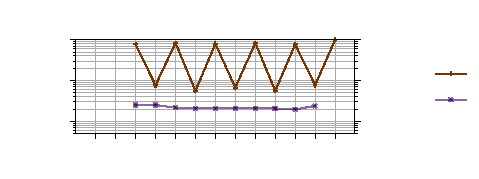
\includegraphics{hamming-single-8}}%
    \gplfronttext
  \end{picture}%
\endgroup

	}
	\vspace{-0.4cm}
	\caption{Comparison of SDC probabilities (lower is better) for Hamming and AN coding for our 8-bit data width example and $A=29$. SDC probabilities for bit flip weights $1$ and $2$ are zero, because both codes always detect these.}
	\label{fig:8bitSDCProbability}
	\vspace{-0.4cm}
\end{figure}

The very good detection capability combined with the easy adaptability of AN coding allows the satisfaction of the requirements \textbf{R2} and \textbf{R3}. The easy adaptability of AN coding means: to detect all $3$ bit flip weights or more, we only have to harden the values with a greater \(A\). This aspect is discussed in the following section in detail. Consequently, AN coding as \emph{error detection-only code} is a very good choice for bit flip detection in database systems allowing to balance detection capability and necessary overhead at run-time. A comparative performance evaluation is done in Section~\ref{sec:MicroBenchmarks}.
